\documentclass{article}
\usepackage[utf8]{inputenc}

\title{AMPTS FTA Electronic Hardware Design}
\author{Matt Ruffner}
\date

\usepackage{url}
\usepackage{array}
\usepackage{float}
\usepackage{natbib}
\usepackage{graphicx}
\usepackage{listings}
\usepackage{fullpage}
\usepackage{hyperref}
\hypersetup{
    colorlinks=true,
    linkcolor=blue,
    filecolor=magenta,      
    urlcolor=cyan,
}

\newcommand{\ddrev}{E}

\begin{document}


\maketitle
\begin{center}
	
\includegraphics[width=4cm]{images/ukcoe.png}
	
\includegraphics[width=4cm]{images/upaero-logo.png}
	
\includegraphics[width=2cm]{images/nasa-logo.png}
	
\includegraphics[width=4cm]{images/ornl.pdf}	
\end{center}
\tableofcontents \newpage
\listoffigures 
\listoftables \newpage



%%%%%%%%%%%%%%%%%%%%%%%%%%%%%%%%%%%%%%%%%%%%%%%%%%%%%%%%%%%%%%%%%%%%%%%%%%%%%%%%%%%%%%%%%
%%%%%%%%%%%%%%%%%%%%%%%%%%%%%%%%%%%%%%%%%%%%%%%%%%%%%%%%%%%%%%%%%%%%%%%%%%%%%%%%%%%%%%%%%
%%%%%%%%%%%%%%%%%%%%%%%%%%%%%%%%%%%%%%%%%%%%%%%%%%%%%%%%%%%%%%%%%%%%%%%%%%%%%%%%%%%%%%%%%
%%%%%%%%%%%%%%%%%%%%%%%%%%%%%%%%%%%%%%%%%%%%%%%%%%%%%%%%%%%%%%%%%%%%%%%%%%%%%%%%%%%%%%%%%
\section{Introduction}
This document outlines the initial design of electrical hardware that will support the flight test article (FTA) being developed for the NASA Flight Opportunities \textit{Additive Manufacturing of Thermal Protection Systems} (AMTPS) project. This project is a collaboration between several NASA facilities including JSC and Langley as well as other research institutions including the University of Kentucky and Oak Ride National Laboratories. Figure \ref{fig:capsule-overview} shows a general overview of the various components that are  expected to be a part of the flight test article (referred to as 'the capsule') based on current requirements.

Capsule hardware must be capable of robust data acquisition in order to characterize the thermal, pressure, and overall heating environment of supersonic reentry. In addition to collecting multiple data channels, the hardware must be capable of transmitting its location as it about to touch back down to Earth. The multichannel data acquisition system must also save flight data for analysis after it touches back down. Timing the deployment of a parachute before touchdown is also a requirement of the hardware in order to lessen the force of impact.

This document is organized as follows: Section \ref{sec:requirements} discusses needed capabilities set by the NASA project design document (rev. \ddrev ) that are relevant to the avionics hardware. Section \ref{sec:ss-design} displays the preliminary designs and testing hardware for the various subsystems of the capsule. This includes data acquisition, logging, and vehicle-to-ground communication for recovery operations. Appendix \ref{appa} contains schematics for PCBs that have been prototyped. Appendix \ref{appb} contains images of testing hardware that has been developed. 

\begin{figure}[h!]
	\centering
	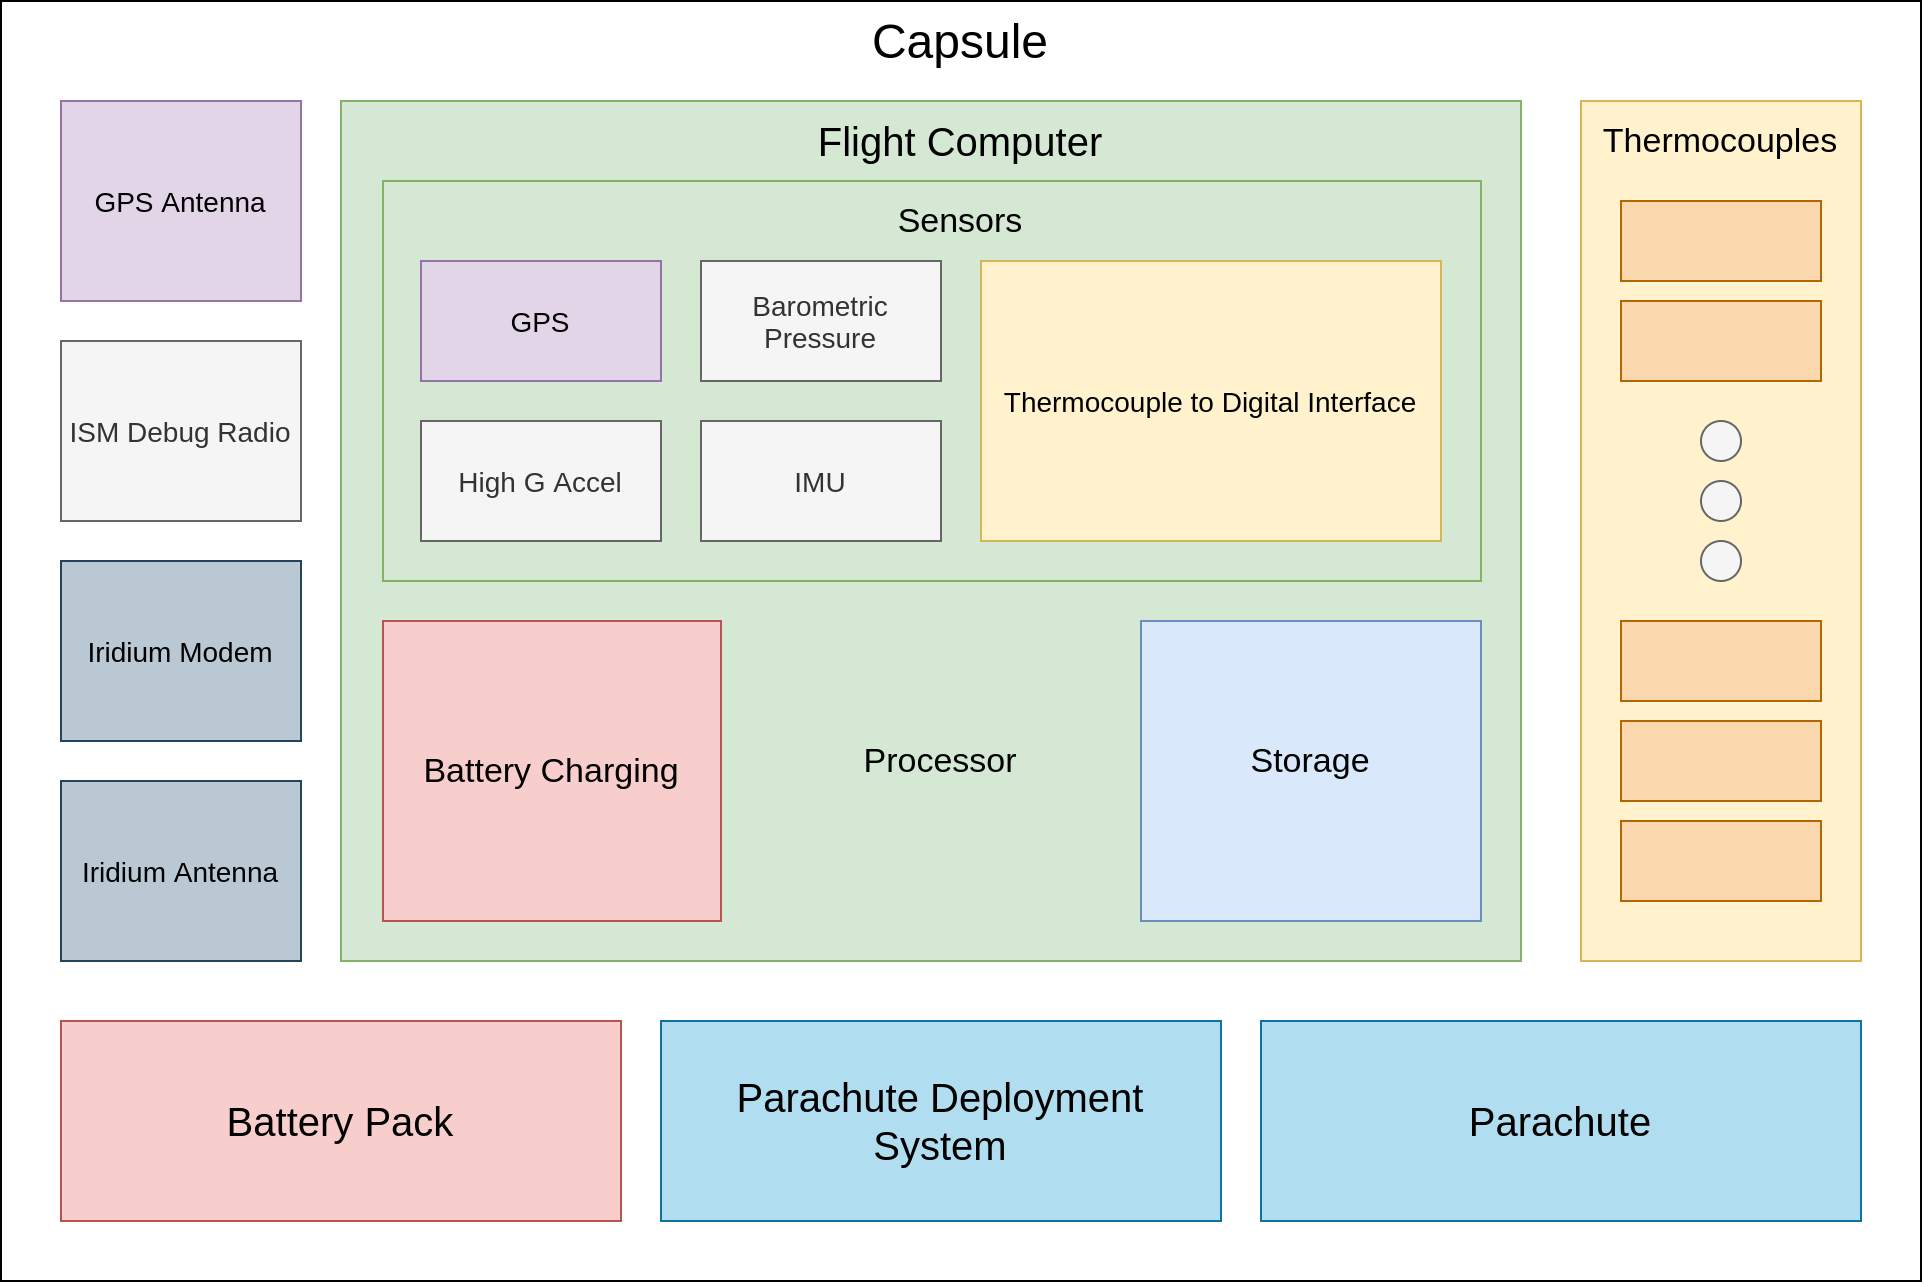
\includegraphics[width=\textwidth]{images/amtps-avionics.png}
	\caption{Capsule component overview, showing the various functional blocks.}
	\label{fig:capsule-overview}
\end{figure}


%%%%%%%%%%%%%%%%%%%%%%%%%%%%%%%%%%%%%%%%%%%%%%%%%%%%%%%%%%%%%%%%%%%%%%%%%%%%%
%%%%%%%%%%%%%%%%%%%%%%%%%%%%%%%%%%%%%%%%%%%%%%%%%%%%%%%%%%%%%%%%%%%%%%%%%%%%%
%%%%%%%%%%%%%%%%%%%%%%%%%%%%%%%%  APPENDIX
%%%%%%%%%%%%%%%%%%%%%%%%%%%%%%%%%%%%%%%%%%%%%%%%%%%%%%%%%%%%%%%%%%%%%%%%%%%%%
%%%%%%%%%%%%%%%%%%%%%%%%%%%%%%%%%%%%%%%%%%%%%%%%%%%%%%%%%%%%%%%%%%%%%%%%%%%%%
\section{Requirements}
\label{sec:requirements}
Based off of the most recent revision (\ddrev) of the flight test requirements document.

\begin{enumerate}
\item Instrumentation and telemetry
  \begin{enumerate}
  \item Shall support betwen 8 and 20 thermocouples of varying type
  \item Shall support up to 6 absolute pressure sensors
  \item Shall support at least 1 intertial measurement unit (IMU)
  \item Should support 1 heat flux sensor
  \item Shall contain a GPS for recovery operations
  \item Telemetry data shall be collected at a minumum of 10Hz
  \item Telemetry data shall be stored to onboard nonvolatile memory that will survive landing
  \item Location telemetry shall be transmitted through a vehicle-to-ground system (e.g. Iridium satellite, Xbee)
  \end{enumerate}
\item Activation and flight sequencing
  \begin{enumerate}
  \item Shall be powered through the duration of the flight
  \item Shall support continuous operation between -20 deg C and 80 deg C
  \item Shall support pre-launch activation on the ground; should support low power mode prior to deployment
  \item Shall detect and/or sense when depoyment has occurred via interfacing with the launch vehicle
  \item Shall trigger parachute deployment at a specified time.
  \end{enumerate}
\end{enumerate}




%%%%%%%%%%%%%%%%%%%%%%%%%%%%%%%%%%%%%%%%%%%%%%%%%%%%%%%%%%%%%%%%%%%%%%%%%%%%%
%%%%%%%%%%%%%%%%%%%%%%%%%%%%%%%%%%%%%%%%%%%%%%%%%%%%%%%%%%%%%%%%%%%%%%%%%%%%%
%%%%%%%%%%%%%%%%%%%%%%%%%%%%%%%%  DESIGN
%%%%%%%%%%%%%%%%%%%%%%%%%%%%%%%%%%%%%%%%%%%%%%%%%%%%%%%%%%%%%%%%%%%%%%%%%%%%%
%%%%%%%%%%%%%%%%%%%%%%%%%%%%%%%%%%%%%%%%%%%%%%%%%%%%%%%%%%%%%%%%%%%%%%%%%%%%%
\section{Preliminary Subsystem Design}
\label{sec:ss-design}

\subsection{Main command and data handling}

Using off the shelf processors for convenience, and also to avoid bottlenecks in prototyping due to unpredictable chip shortages. Currently, two development boards from Adafruit are being used to prototyping and are listed below in Table \ref{tab:processors}\footnote{TPM: Temperature and Pressure Measurement}\footnote{CDH: Command and Data Handling}.

\begin{table}[h!]	
	\caption{List of processors used and their capabilities.}
	\begin{tabular}{l | c c m{5cm}}
		Part & Description & Role & Product Link \\
		\hline
		Feather M0 Basic Proto & Cortex-M0 @ 48 MHz & TPM Processor & \url{https://www.adafruit.com/product/2772}\\
		Feather M4 Express & Cortex-M4 @ 120Mhz & CDH Processor & \url{https://www.adafruit.com/product/3857} 
	\end{tabular}
	\label{tab:processors}
\end{table}

The diagram in Figure \ref{fig:main-overview} provides a general overview of the organization of electronic hardware within the capsule. 
\begin{figure}[h!]
	\centering
	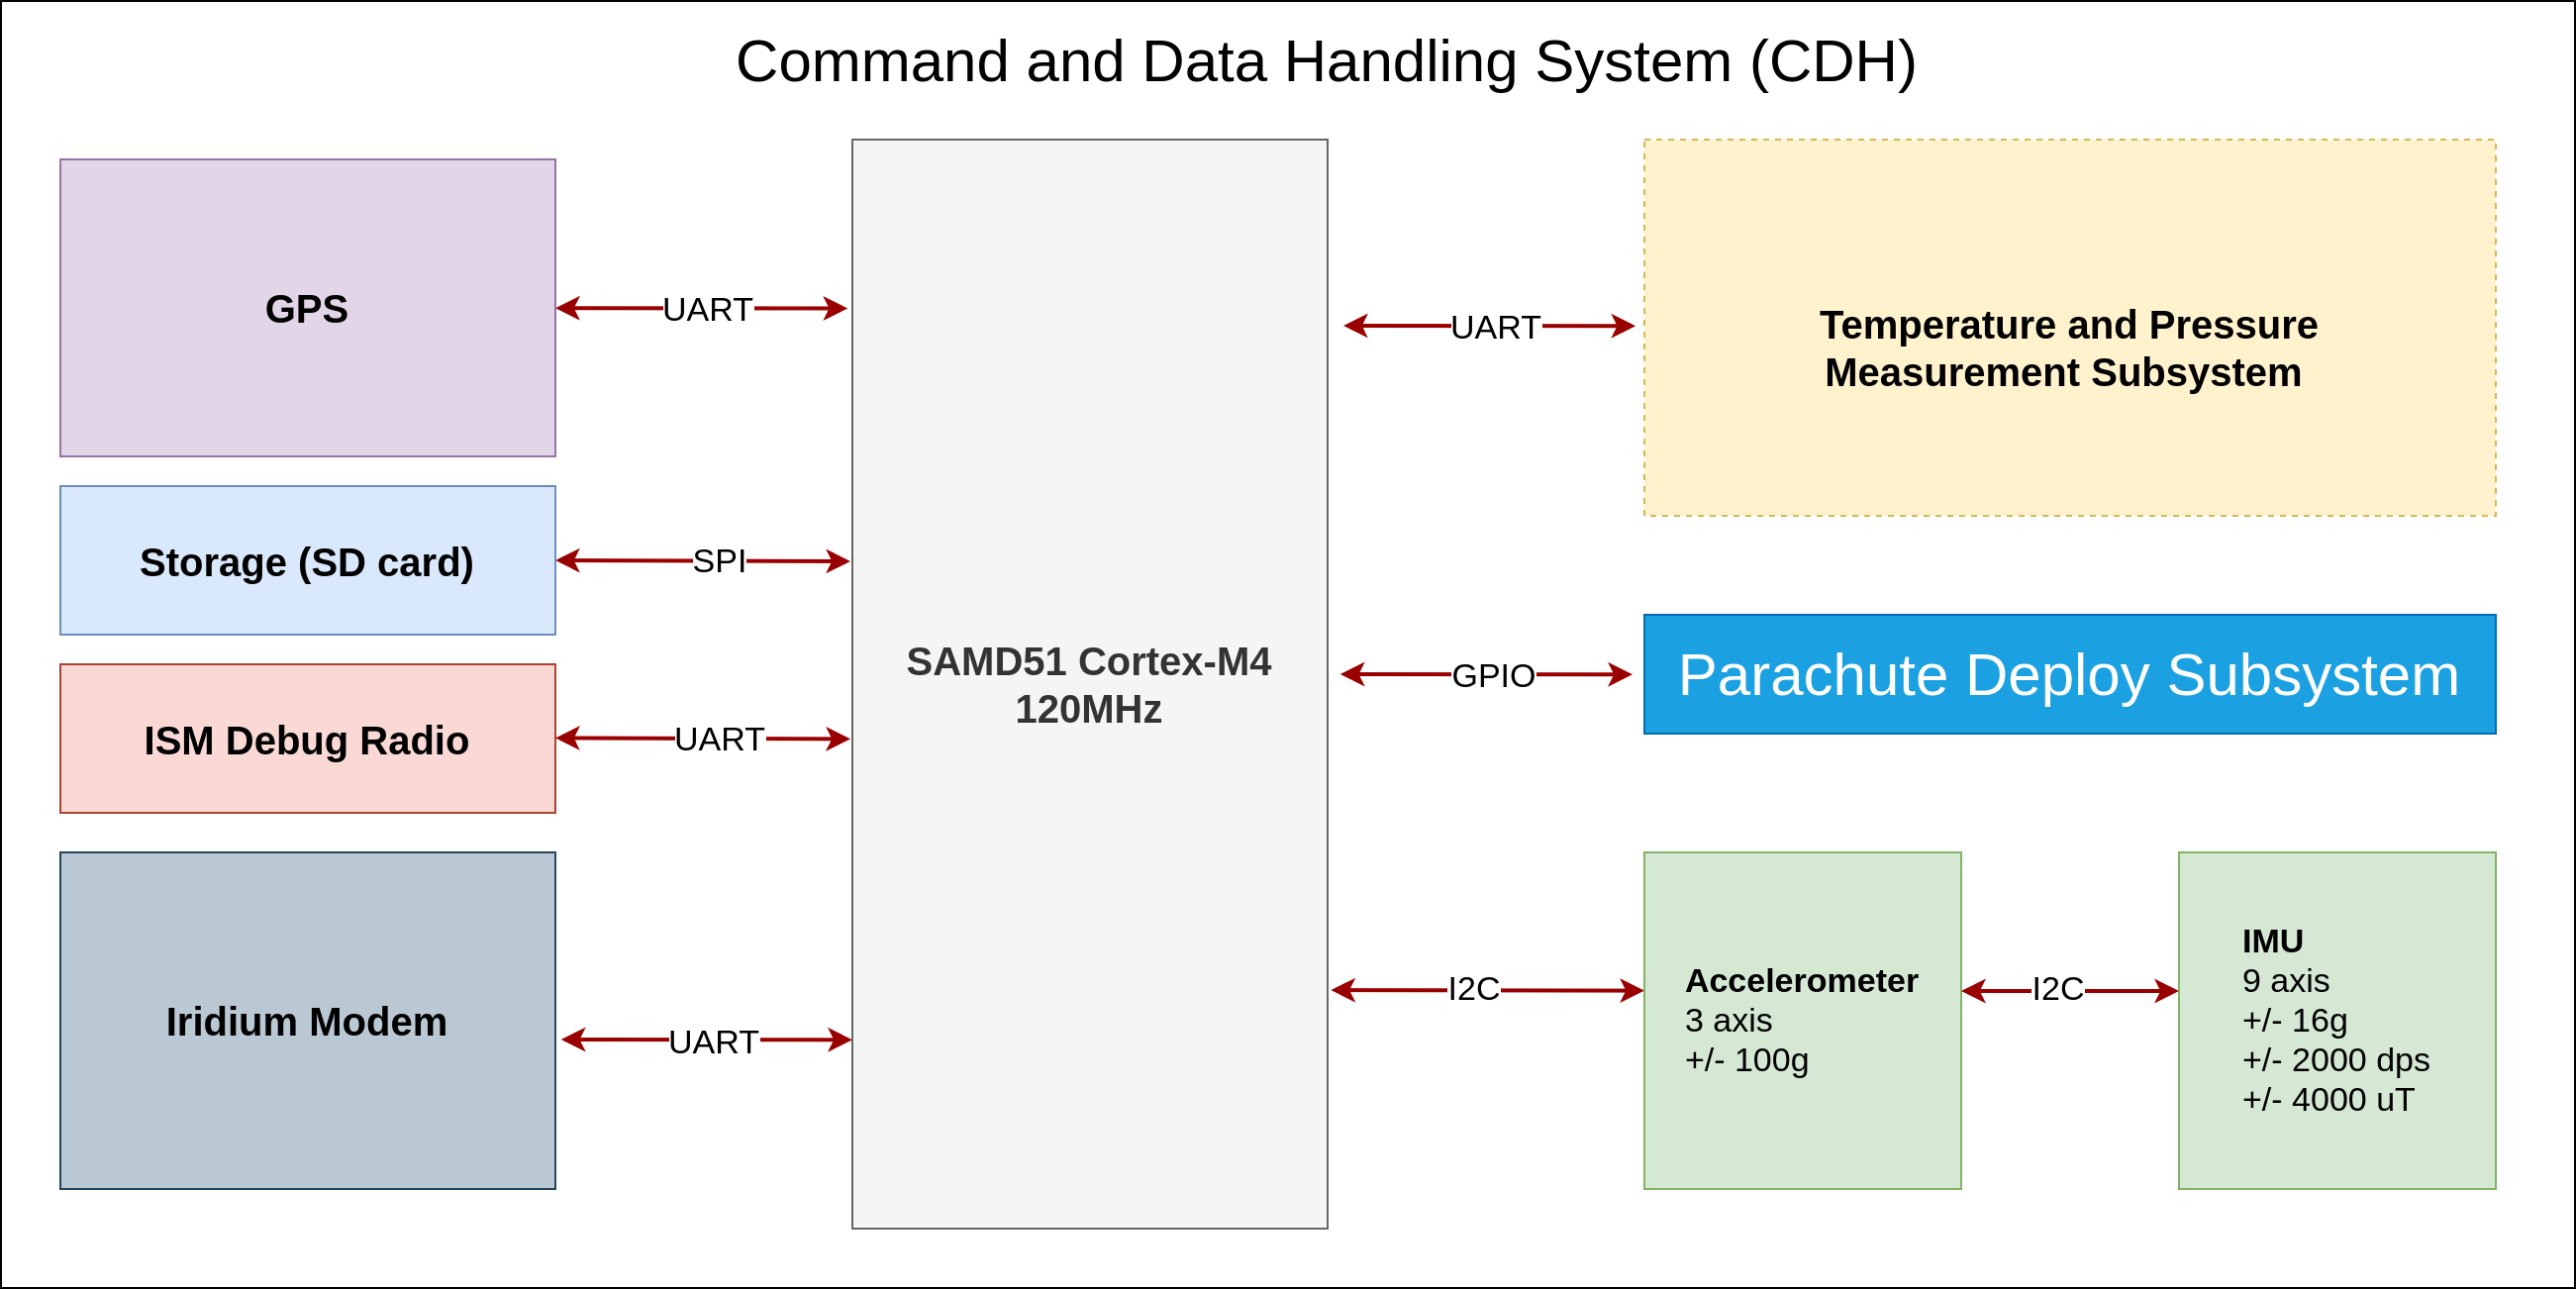
\includegraphics[width=\textwidth]{images/amtps-main-system.png}
	\caption{Main functional components of the capsule and the communication buses between them.}
	\label{fig:main-overview}
\end{figure}


%%%%%%%%%%%%%%%%%%%%%%%%%%%%%%%%%%%%%%%%%%%%%%%%%%%%%%%%%%%%%%%%%%%%%%%%%%%%%
%%%%%%%%%%%%%%%%%%%%%%%%%%%%%%%%%%%%%%%%%%%%%%%%%%%%%%%%%%%%%%%%%%%%%%%%%%%%%
\subsection{Temperature and Pressure Measurement}
The temperature and pressure measurement (TPM) Subsystem (TPMS) supports collection of several datapoints needed for recreating the heating environment of reentry. 


In order to support the large number of TCs required in the capsule, a breakout board supporting 6 of the MCP9600T-E/MX series TC to digital converter was designed. This TC converter chip was selected due to its support for a wide variety of TC types (K, J, T, N, S, E, B and R)\footnote{\url{https://www.digikey.com/en/products/detail/microchip-technology/MCP96L00T-E-MX/9606988}}, as well as its chainable I$^2$C interface, allowing more sensing elements to connected with less wiring (similar SPI based conversion chips have a chip select line per chip that would restrict the number of pins available for other capsule functionality).

A breakout board was designed with 6 MCP9600 converter chips to serve as an initial design for a t ewill be done on a breakout 


For pressure meausrement, Honeywell sensing solutions temperature compensated absolution digital pressure sensors were selected and are shown in Table \ref{tab:pressure-sensors}. These single port absolute pressure sensors are available with a variety of sensitivities, allowing a different sensor to be exchanged later on in the design process if it is determined that the current predicted pressure environment is no longer accurate.

A picture of the preliminary pressure sensor evaluative setup in shown in Appendix \ref{appb}, Figure \ref{fig:pressure-testbed}.

\begin{table}[h!]
	\caption{List of pressure sensors and their capabilities}
	\begin{tabular}{c | c m{9cm}}
		Part & Measurement Range & Product Link \\
		\hline
		SSCSRNN015PA3A3 & 0-103.42 kPa & \url{https://www.digikey.com/en/products/detail/honeywell-sensing-and-productivity-solutions/SSCSRNN015PA3A3/2416212}\\
		SSCSRNN1-6BA7A3 & 0-160 kPa & \url{https://www.digikey.com/en/products/detail/honeywell-sensing-and-productivity-solutions/SSCSRNN1-6BA7A3/2416214} 
	\end{tabular}
\label{tab:pressure-sensors}
\end{table}

Finally, Figure \ref{fig:tpms-overview} shows an overview of the temperature and pressure monitoring subsystem

\begin{figure}[h!]
	\centering
	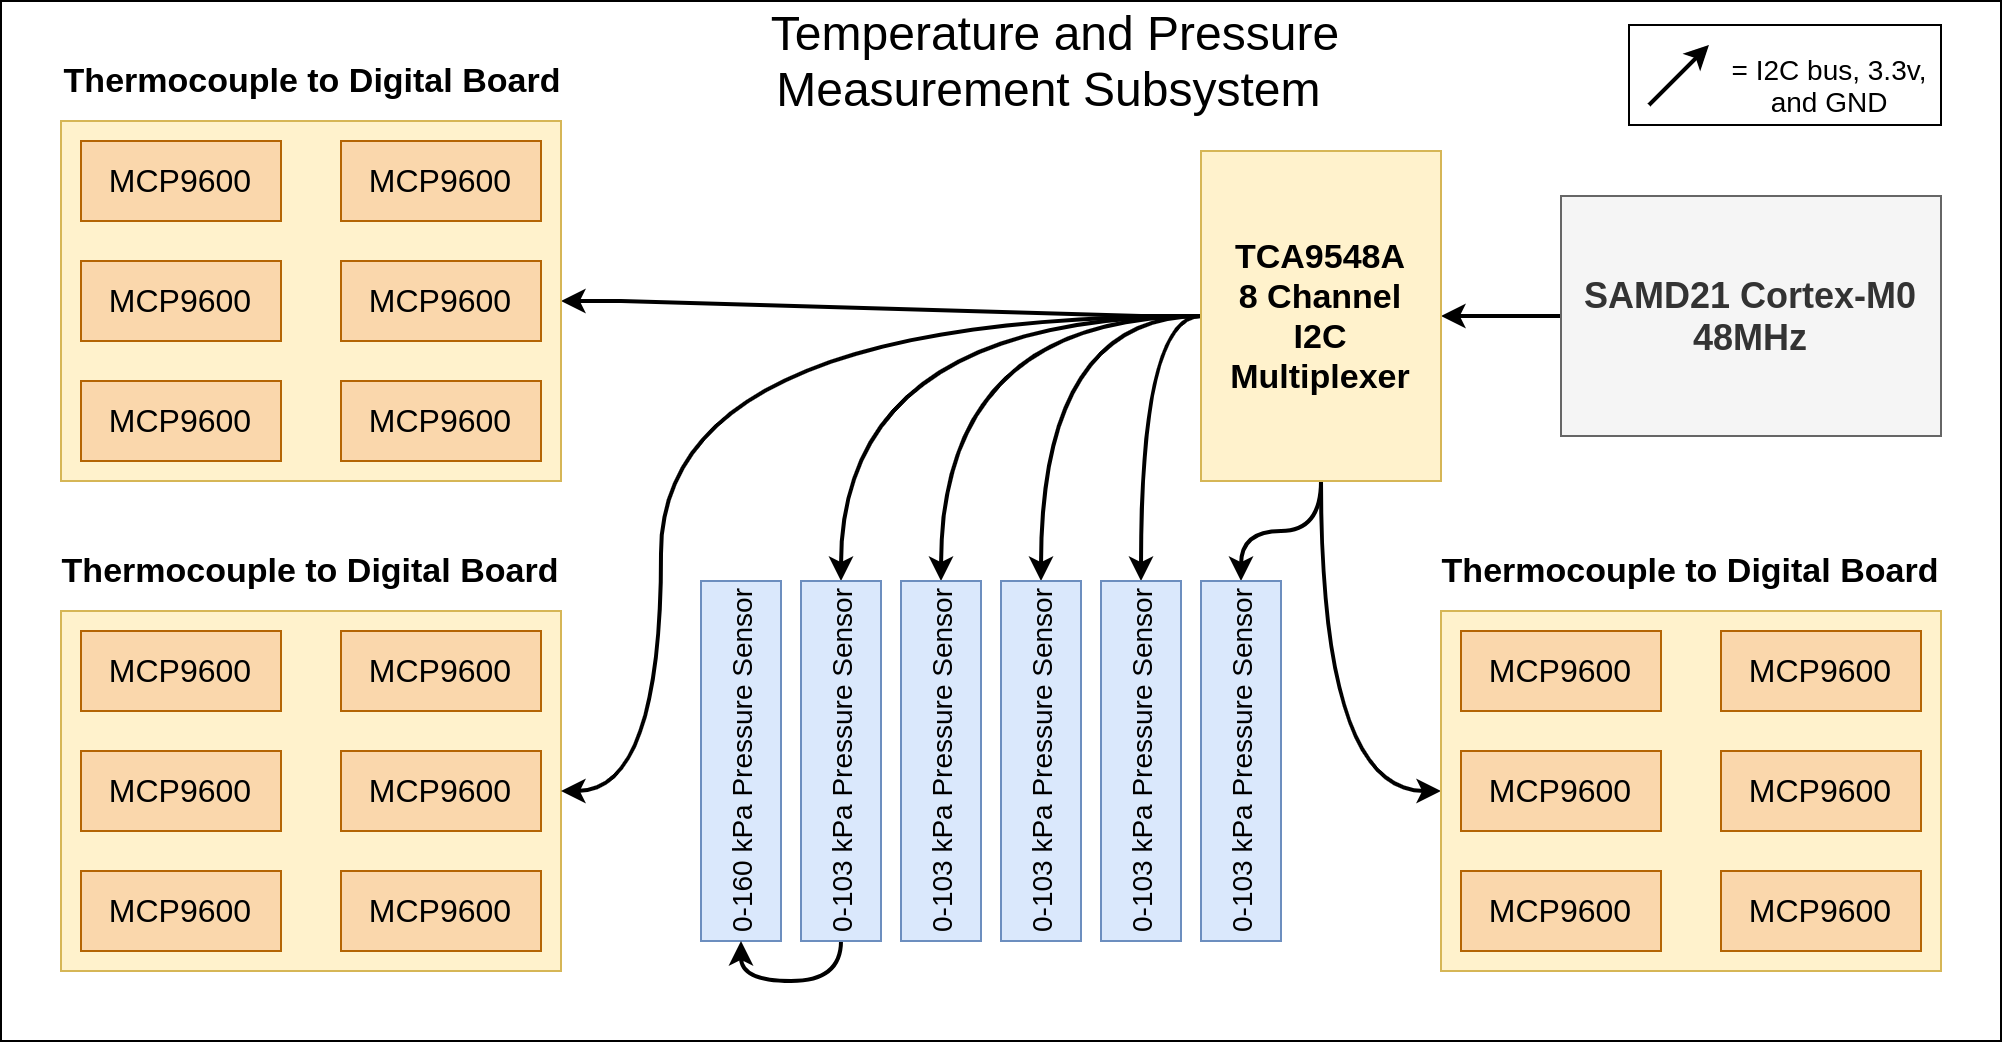
\includegraphics[width=\textwidth]{images/amtps-temp-pressure-subsystem.png}
	\caption{Overview of the TPMS.}
	\label{fig:tpms-overview}
\end{figure}


\subsection{Inertial Measurement}
A breakout board for the H3LIS100DL~\footnote{\url{https://www.digikey.com/en/products/detail/stmicroelectronics/H3LIS100DL/7313278}} +/- 100g accelerometer has been designed to help in the evaluation of this IC as an effective way to measure acceleration loads on the capsule. The ADXL377 is another potential high-g 3-axis acceleromter~\footnote{\url{https://www.adafruit.com/product/1413}}, but has analog output and higher cost since it is currently only available in a pre-assembled breakout board.

In addition to a high-g 3-axis accelerometer, a lower dynamic range 6 axis acceleromter+gyroscope chip will also be included in the capsule (such as a ICM-20949 or MPU6050).

%%%%%%%%%%%%%%%%%%%%%%%%%%%%%%%%%%%%%%%%%%%%%%%%%%%%%%%%%%%%%%%%%%%%%%%%%%%%%
%%%%%%%%%%%%%%%%%%%%%%%%%%%%%%%%%%%%%%%%%%%%%%%%%%%%%%%%%%%%%%%%%%%%%%%%%%%%%
\subsection{Telemetry}

Iridium modem to send GPS coordinates for recovery operations. University of Kentucky has an Iridium modem available to use, with an account providing message credits. Discussion on the use of this modem is yet to have happened. Additional vehicle-to-ground telemetry would be reassuring as the Iridium network can be unreliable for short periods of time. It is unclear whether this would be achievable with a COTS radio link (such as XBee or LORA) that would not require FCC certification. This requires coordination with launch site for tracking with a directional antenna and other hardware setup. The appeal of the Iridium is we get an email with the GPS coordinates of the capsule and we can tell the recovery crew the location of the capsule from anywhere. 

%%%%%%%%%%%%%%%%%%%%%%%%%%%%%%%%%%%%%%%%%%%%%%%%%%%%%%%%%%%%%%%%%%%%%%%%%%%%%
%%%%%%%%%%%%%%%%%%%%%%%%%%%%%%%%%%%%%%%%%%%%%%%%%%%%%%%%%%%%%%%%%%%%%%%%%%%%%
\subsection{Storage}
On board non-volatile storage is required to log in-flight telemetry data for post processing. Due to the high vibrational loads expected during launch, an SD card might be unreliable (spring loaded contacts could separate from card). For this reason, solid state flash integrated circuits are being explored that can store just as much information as an SD card. 

Exporting logged data from the capsule would then be done via cabled connection to a computer after capsule recovery.


%%%%%%%%%%%%%%%%%%%%%%%%%%%%%%%%%%%%%%%%%%%%%%%%%%%%%%%%%%%%%%%%%%%%%%%%%%%%%
%%%%%%%%%%%%%%%%%%%%%%%%%%%%%%%%%%%%%%%%%%%%%%%%%%%%%%%%%%%%%%%%%%%%%%%%%%%%%
\section{Other Considerations}

\subsection{Durability}
Syntactic foam may be used. Consisting of glass microballoons with epoxy resin, it can encase electronics to protect from very high acceleration loads during ascent. Currently working with NASA JSC to get glass microballoons to UK for testing.


\subsection{Cost}
According the the most recent revision of the project outline, NASA has alotted \$3,000 towards the avionics design. Currently the University of Kentucky has not used any of these funds in the prototyping of capsule hardware.








%%%%%%%%%%%%%%%%%%%%%%%%%%%%%%%%%%%%%%%%%%%%%%%%%%%%%%%%%%%%%%%%%%%%%%%%%%%%%
%%%%%%%%%%%%%%%%%%%%%%%%%%%%%%%%%%%%%%%%%%%%%%%%%%%%%%%%%%%%%%%%%%%%%%%%%%%%%
%%%%%%%%%%%%%%%%%%%%%%%%%%%%%%%%  APPENDIX
%%%%%%%%%%%%%%%%%%%%%%%%%%%%%%%%%%%%%%%%%%%%%%%%%%%%%%%%%%%%%%%%%%%%%%%%%%%%%
%%%%%%%%%%%%%%%%%%%%%%%%%%%%%%%%%%%%%%%%%%%%%%%%%%%%%%%%%%%%%%%%%%%%%%%%%%%%%
\appendix


\section{Schematics}
\label{appa}

\subsection{Command and Data Handling}
Schematics for the Cortex-M0/M4 development boards are available from the links provided to the Adafruit product pages.

\subsection{TC breakout board}

\begin{figure}[H]
	\centering
	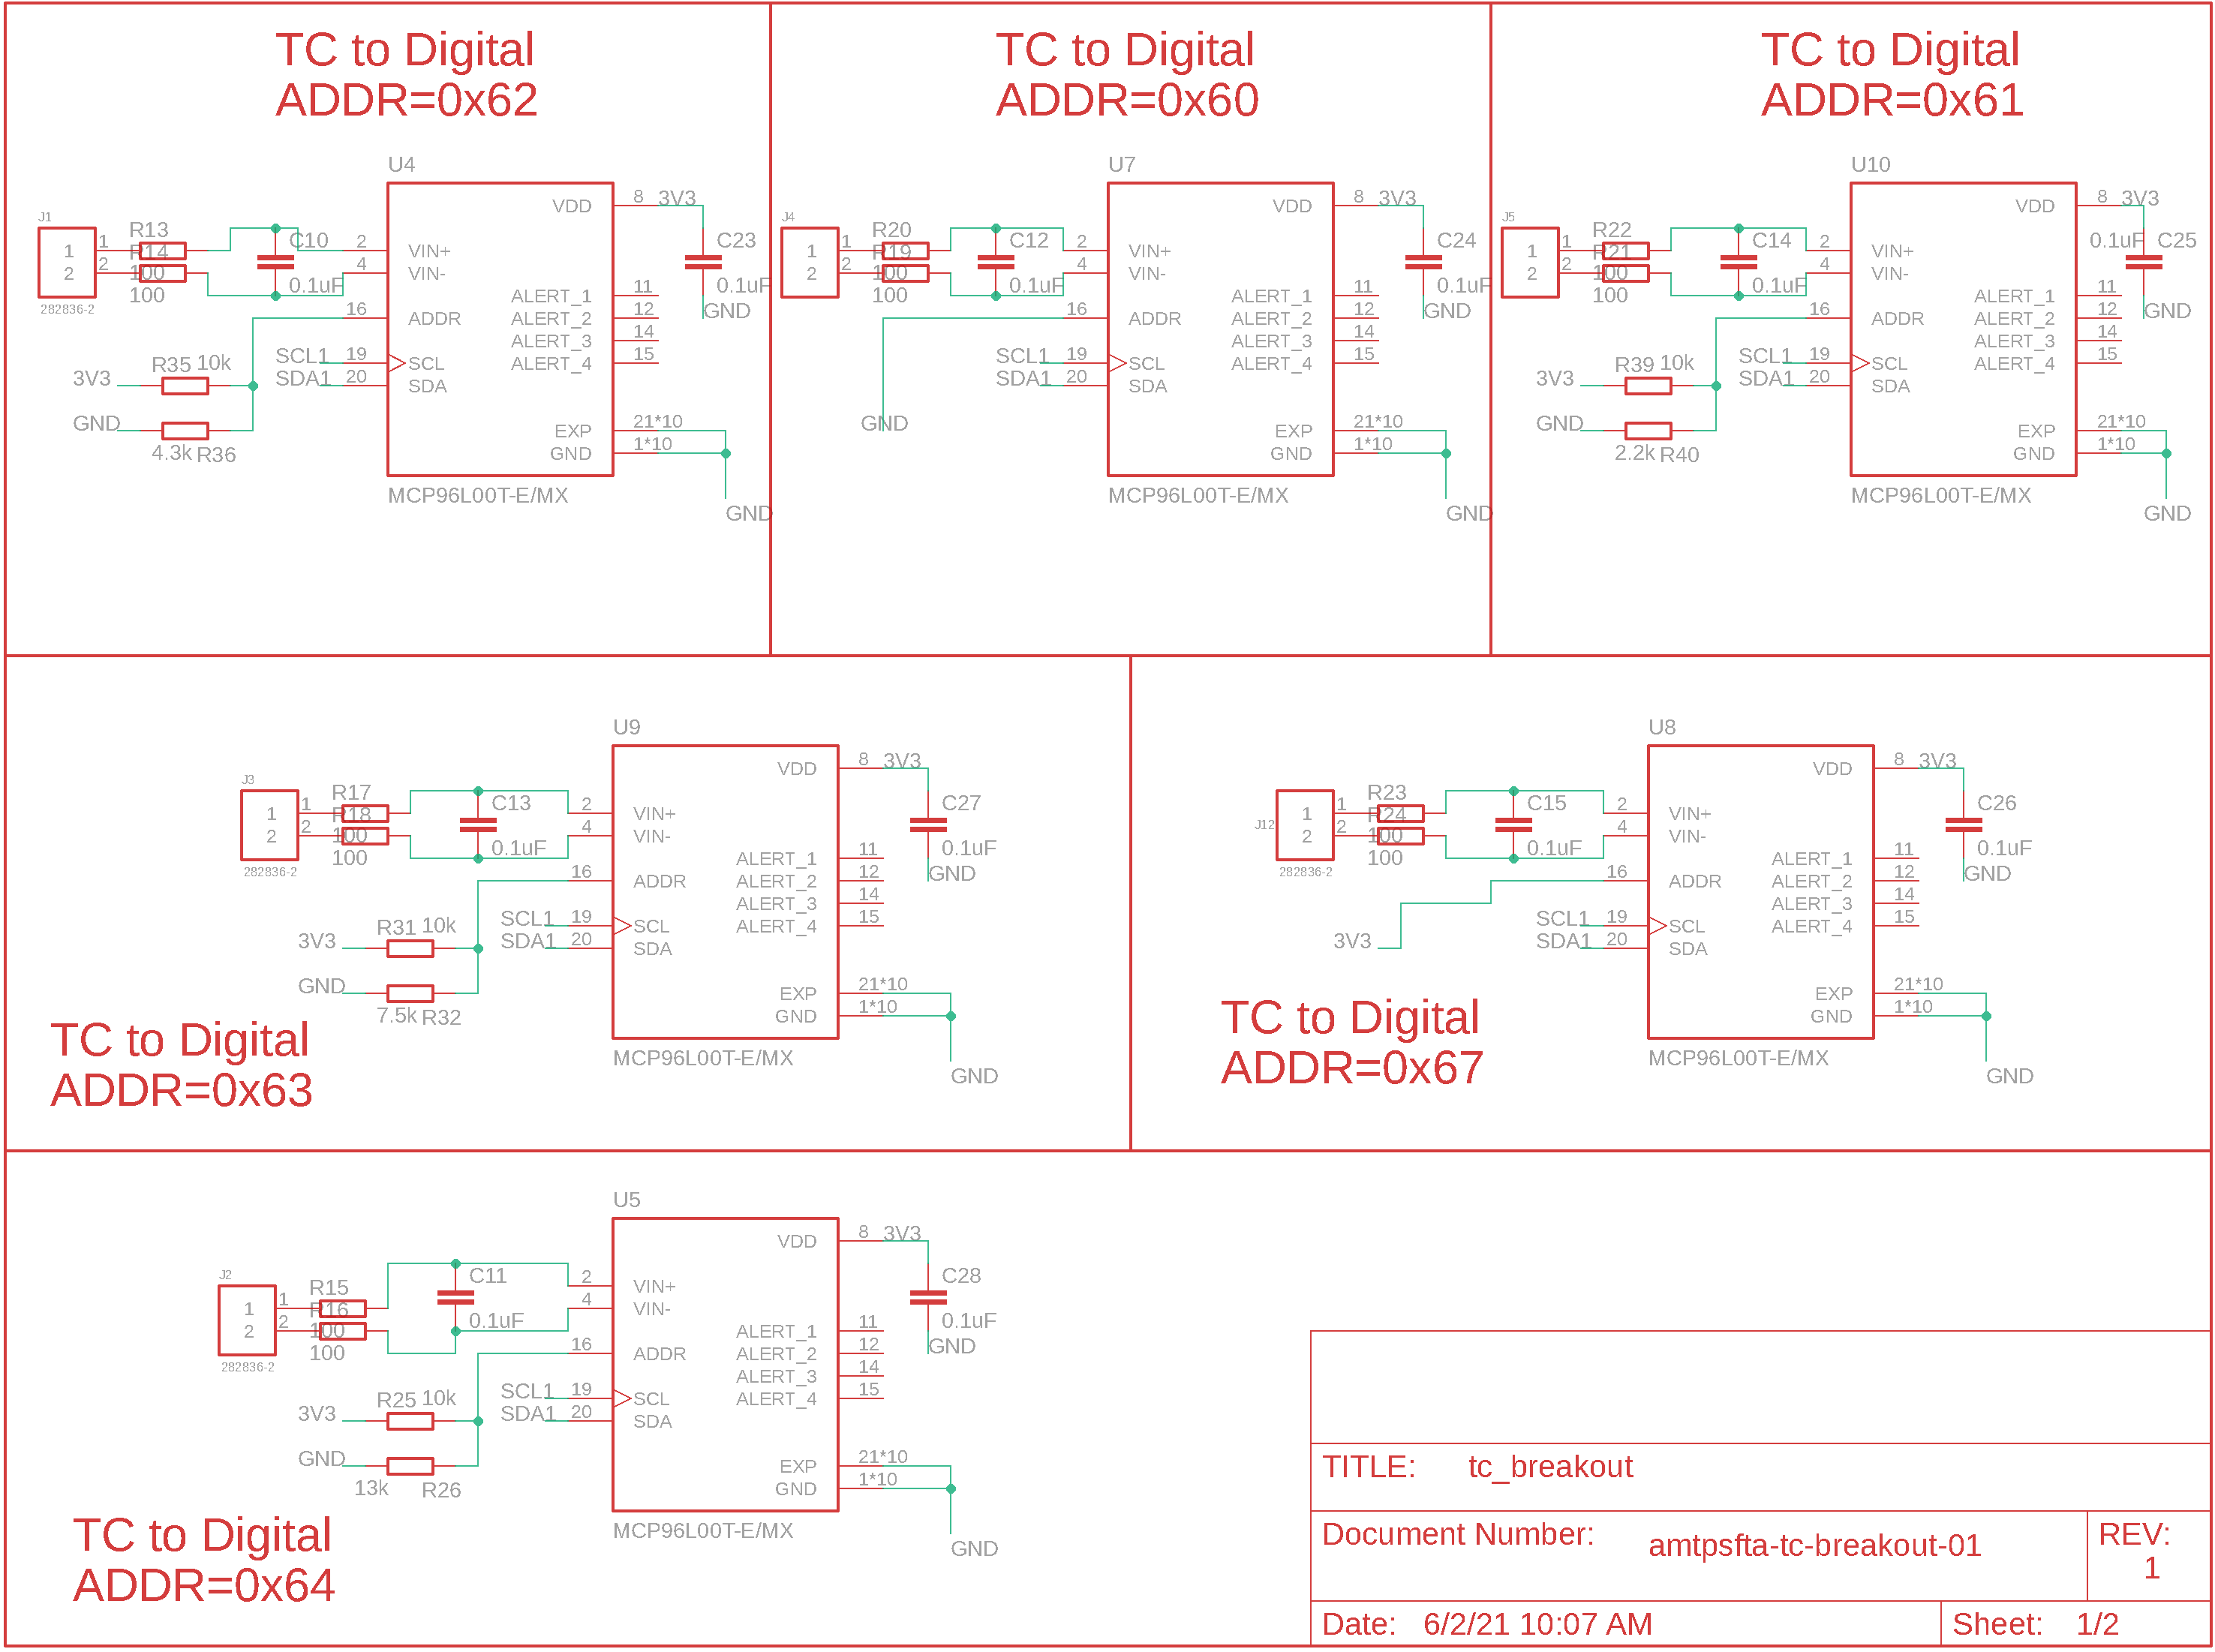
\includegraphics[width=\textwidth]{images/tc-breakout-p1}
	\label{fig:schematic-tc-breakout-p1}
\end{figure}

\begin{figure}[H]
	\centering
	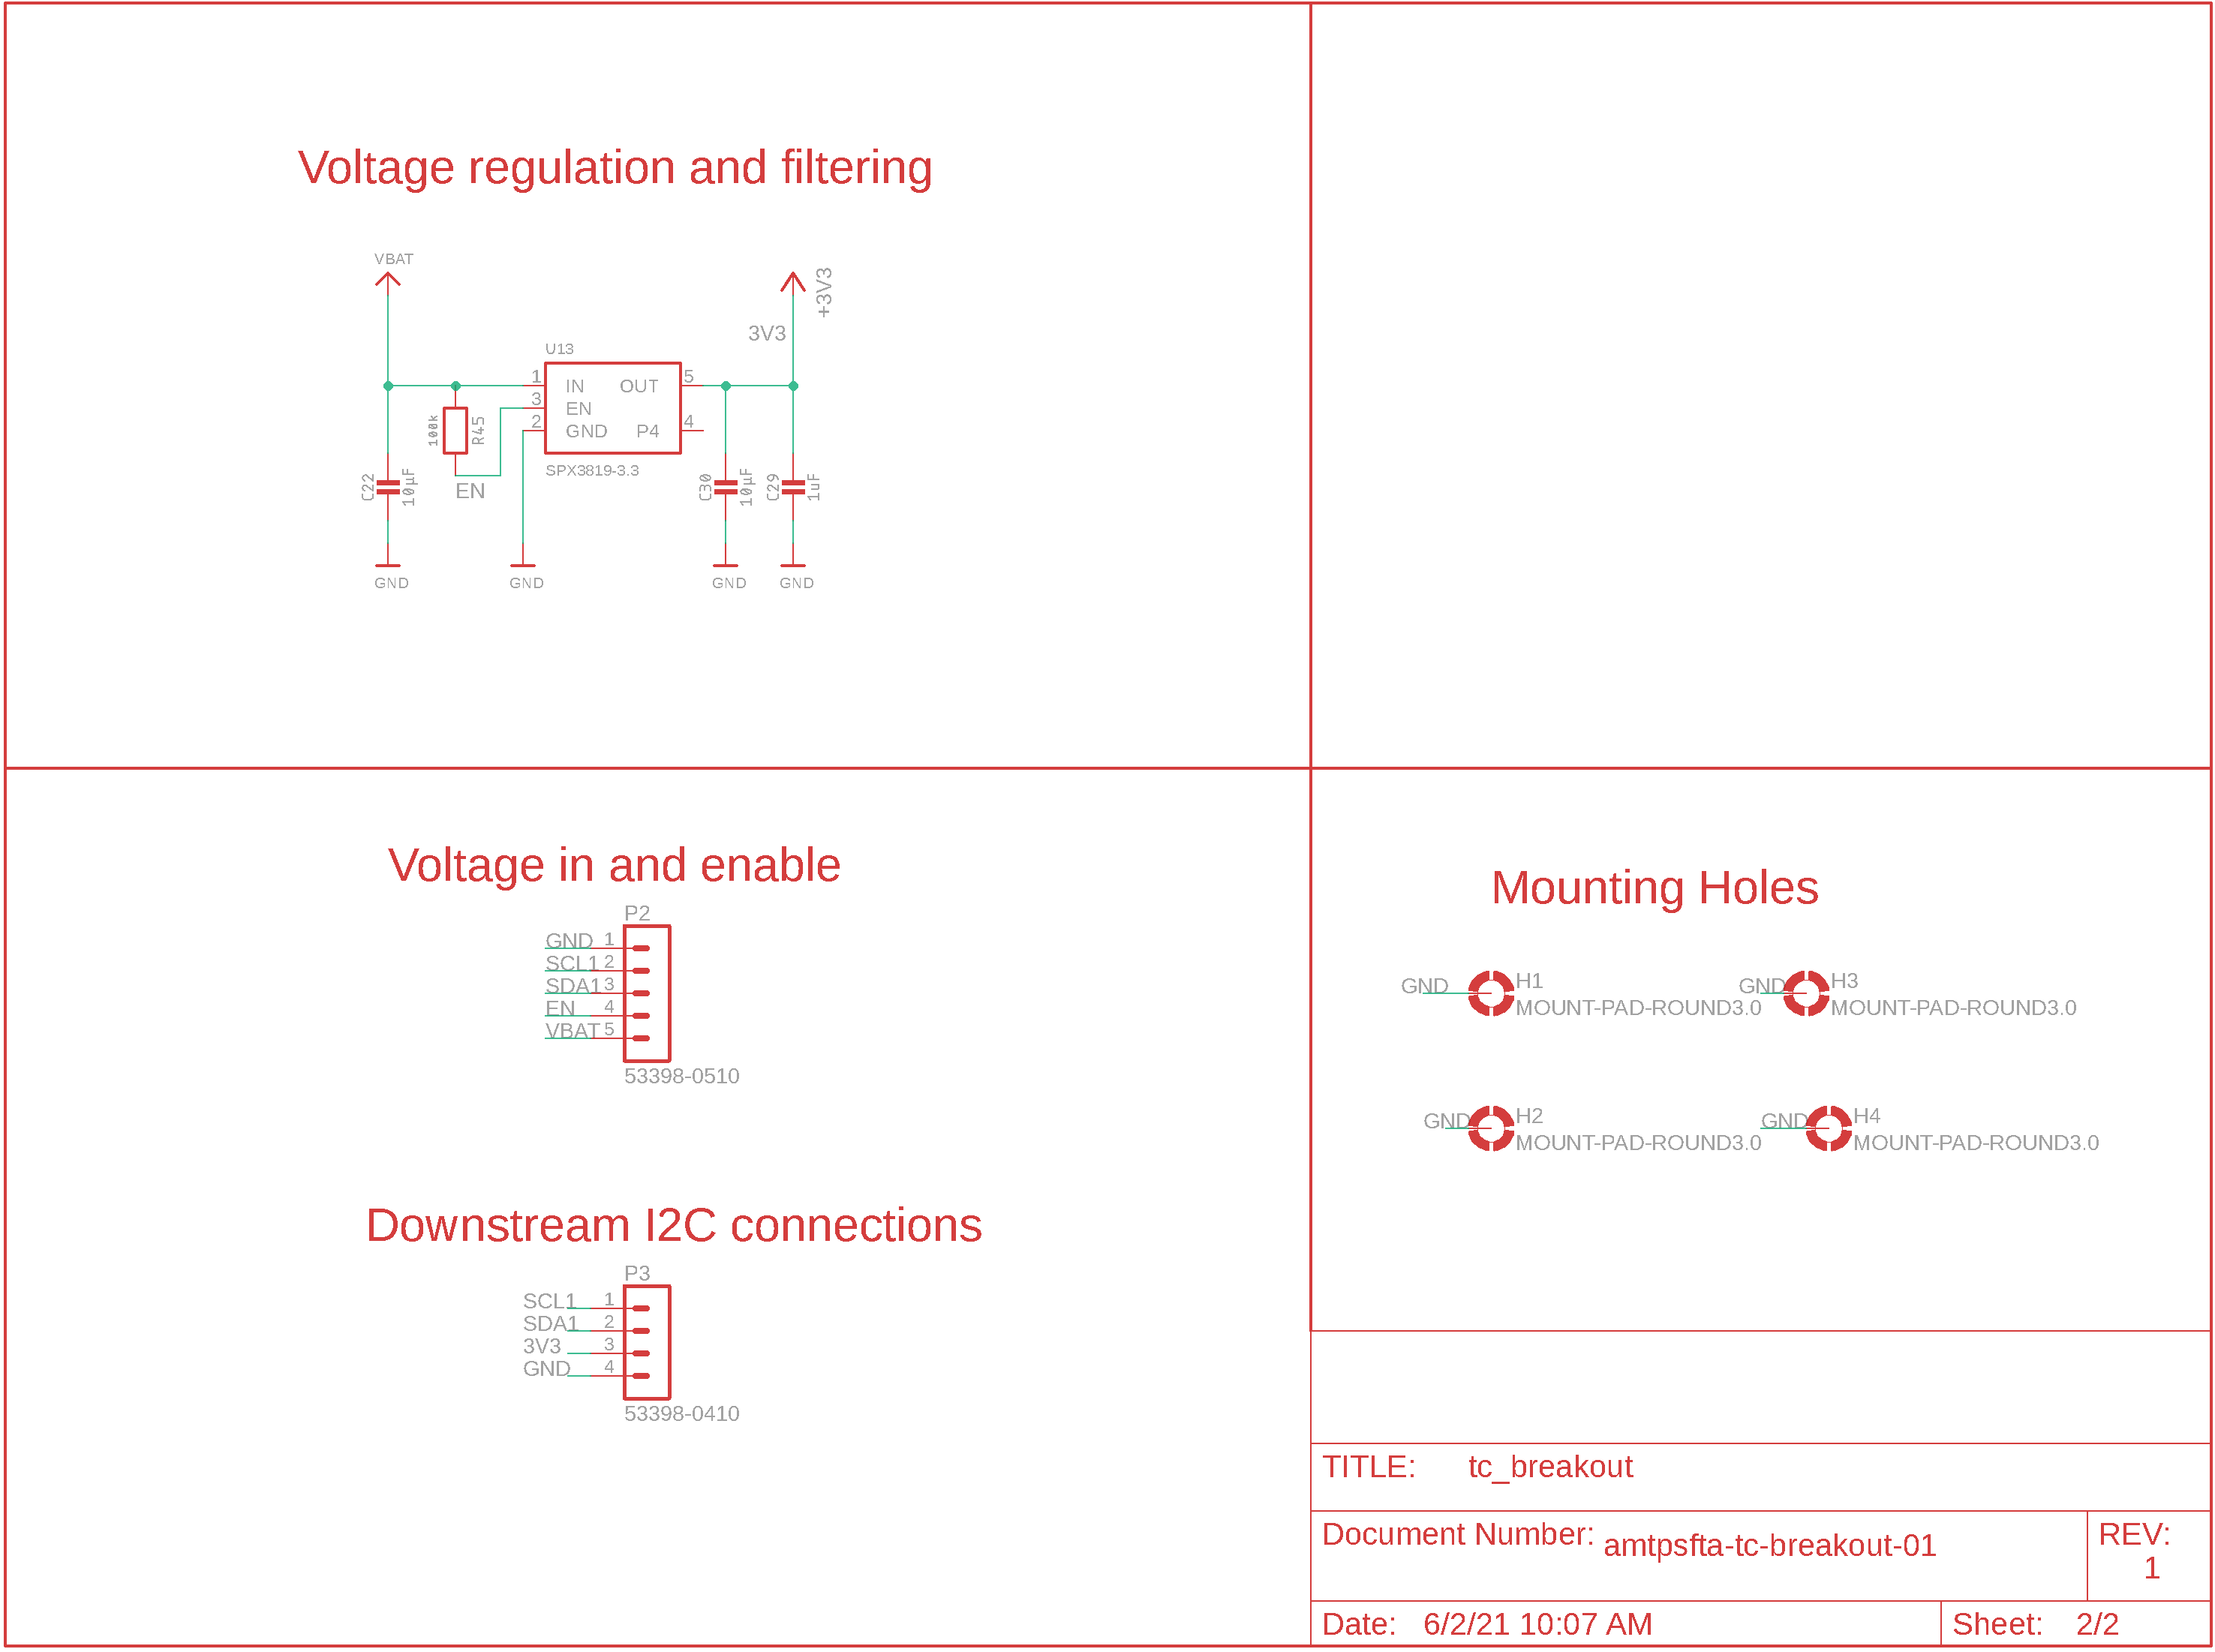
\includegraphics[width=\textwidth]{images/tc-breakout-p2}
	\label{fig:schematic-tc-breakout-p2}
\end{figure}


\section{Testing setup}
\label{appb}

\begin{figure}[H]
	\centering
	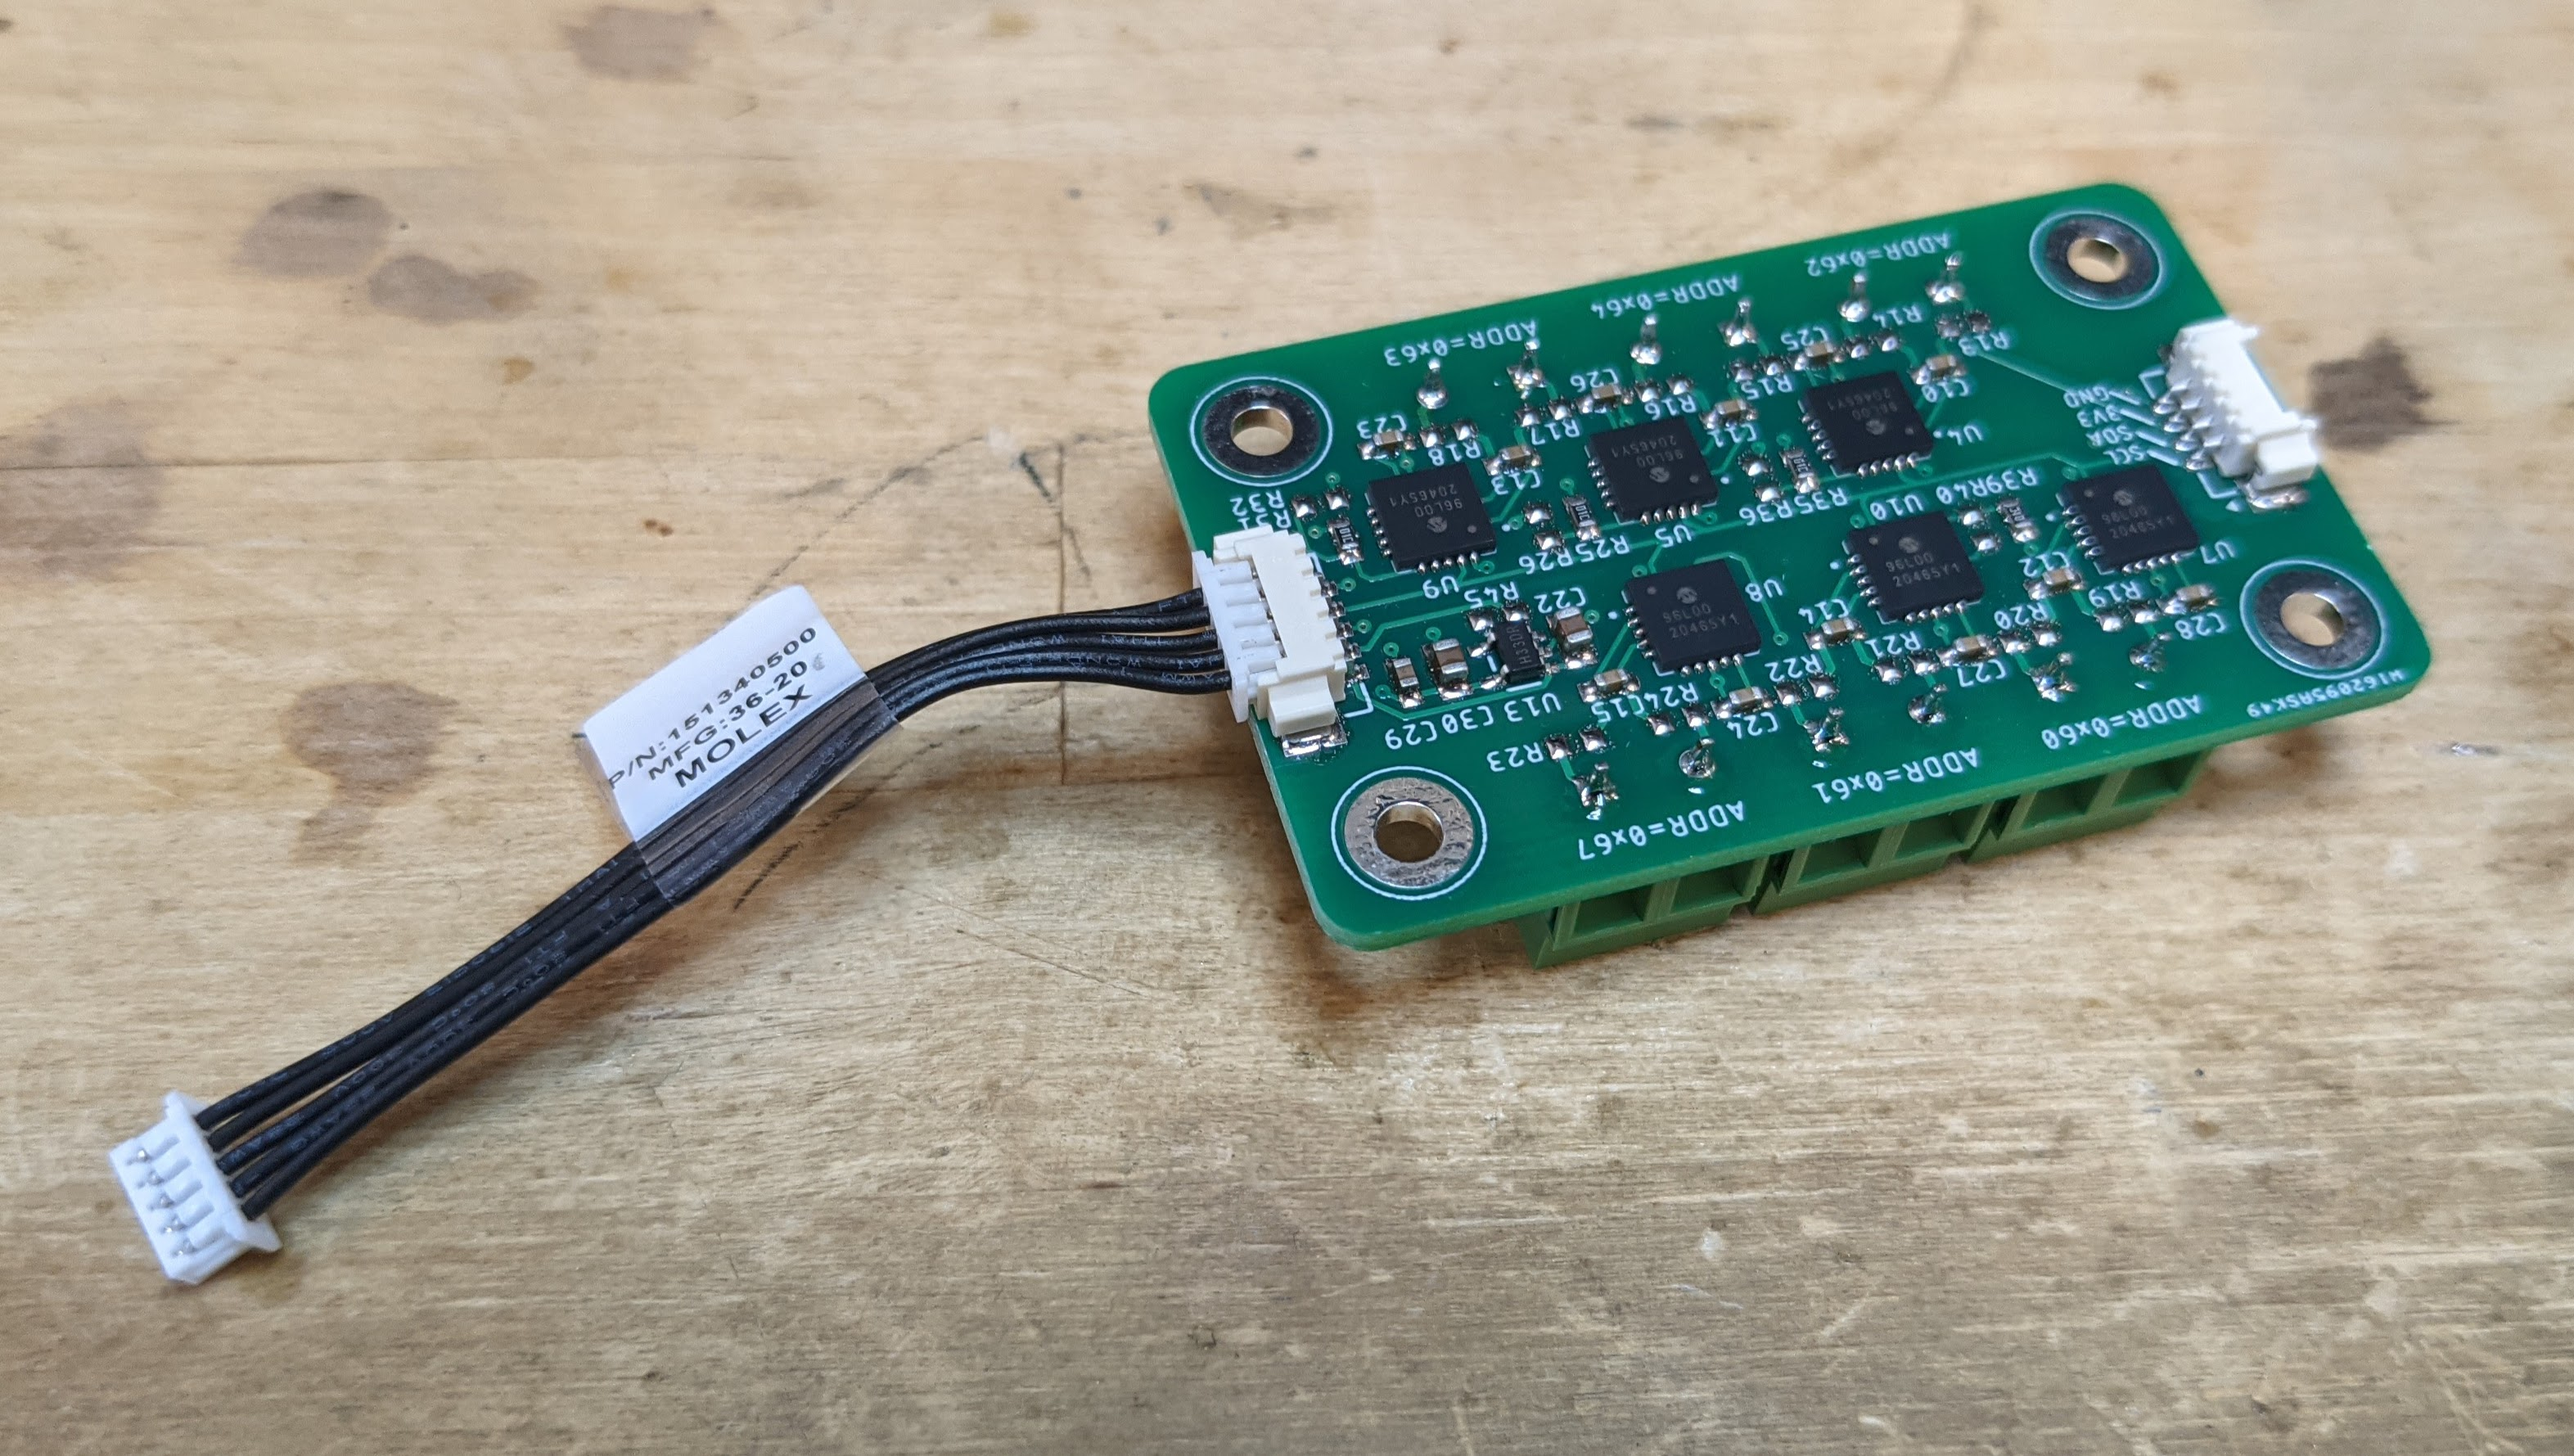
\includegraphics[width=\textwidth]{images/tc-board-bottom}
	\caption{Bottom of V1 Evaluation board for MCP9600 TC to digital converter}
	\label{fig:tc-board-bottom}
\end{figure}

\begin{figure}[h!]
	\centering
	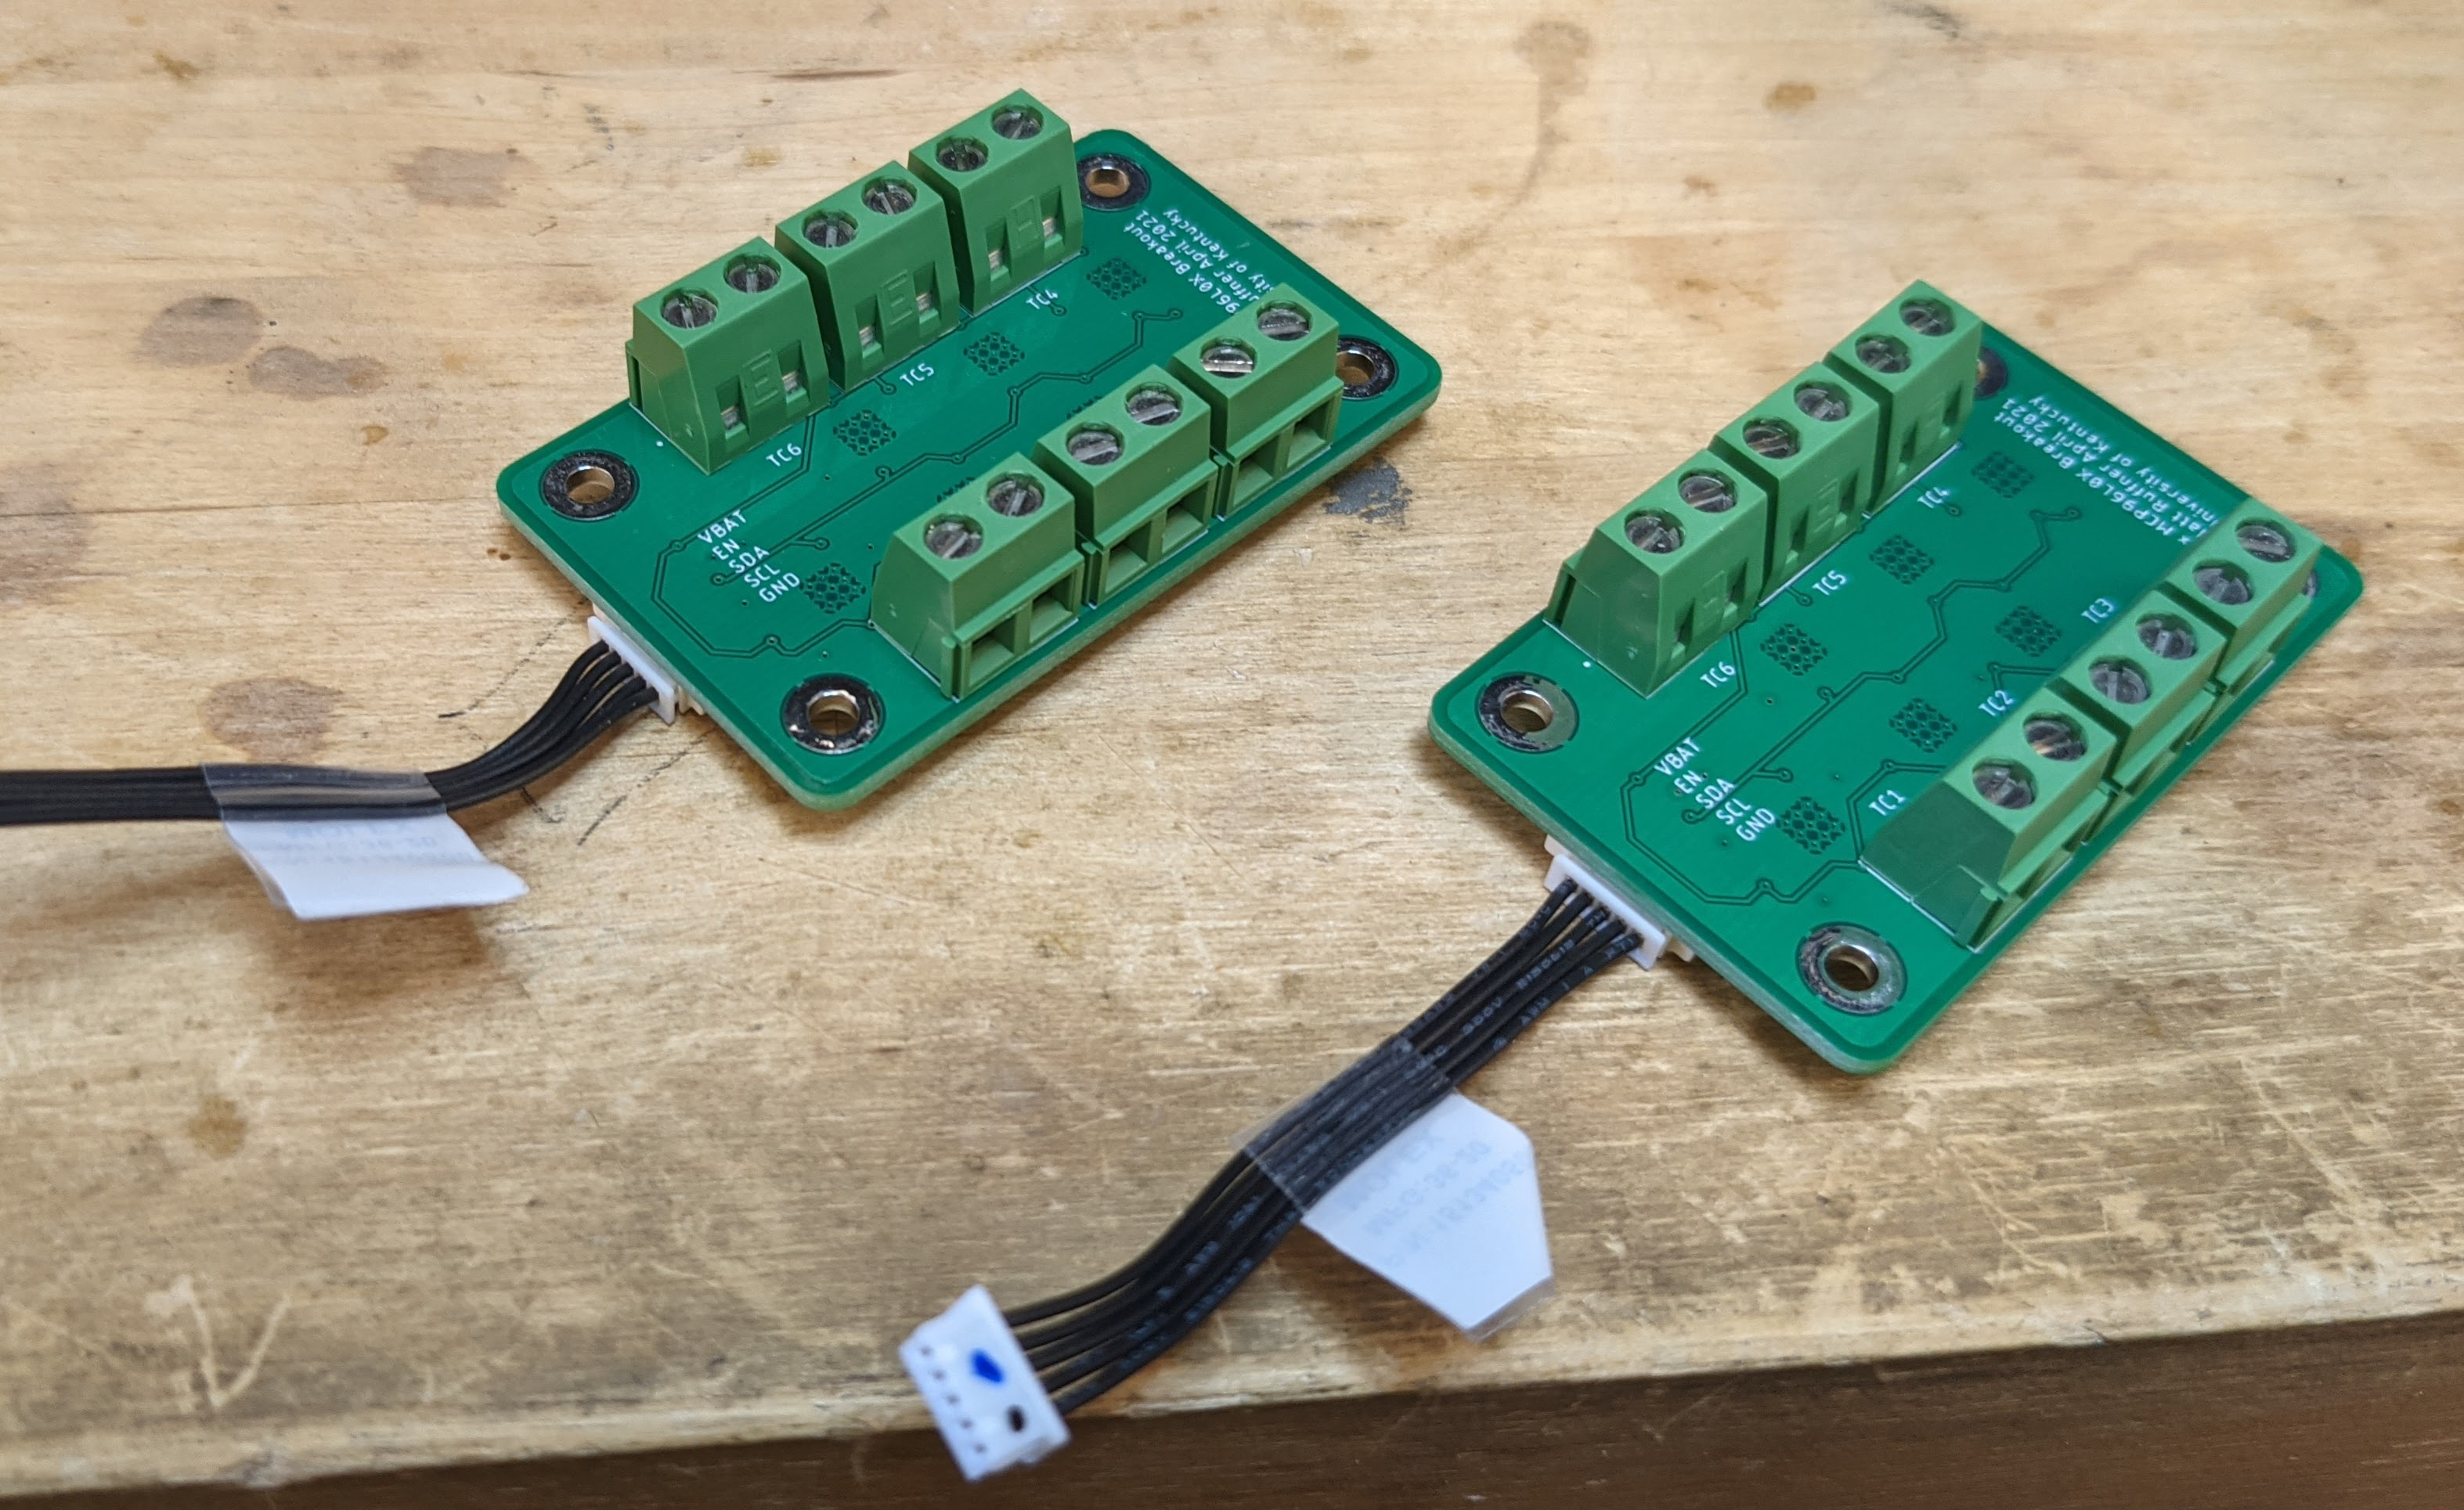
\includegraphics[width=\textwidth]{images/tc-board-top}
	\caption{Top of V1 Evaluation board for MCP9600 TC to digital converter}
	\label{fig:tc-board-top}
\end{figure}

\begin{figure}[h!]
	\centering
	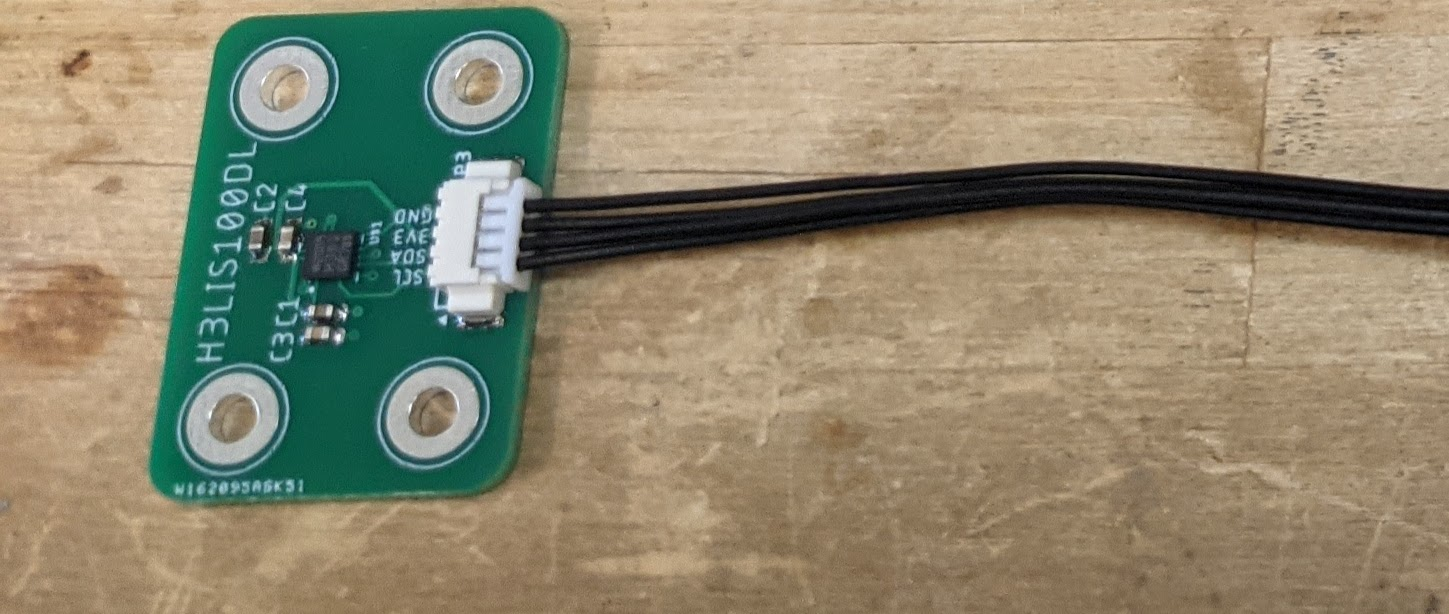
\includegraphics[width=\textwidth]{images/100g-accel-board}
	\caption{High g accelerometer testing PCB.}
	\label{fig:accel-board}
\end{figure}

\begin{figure}[h!]
	\centering
	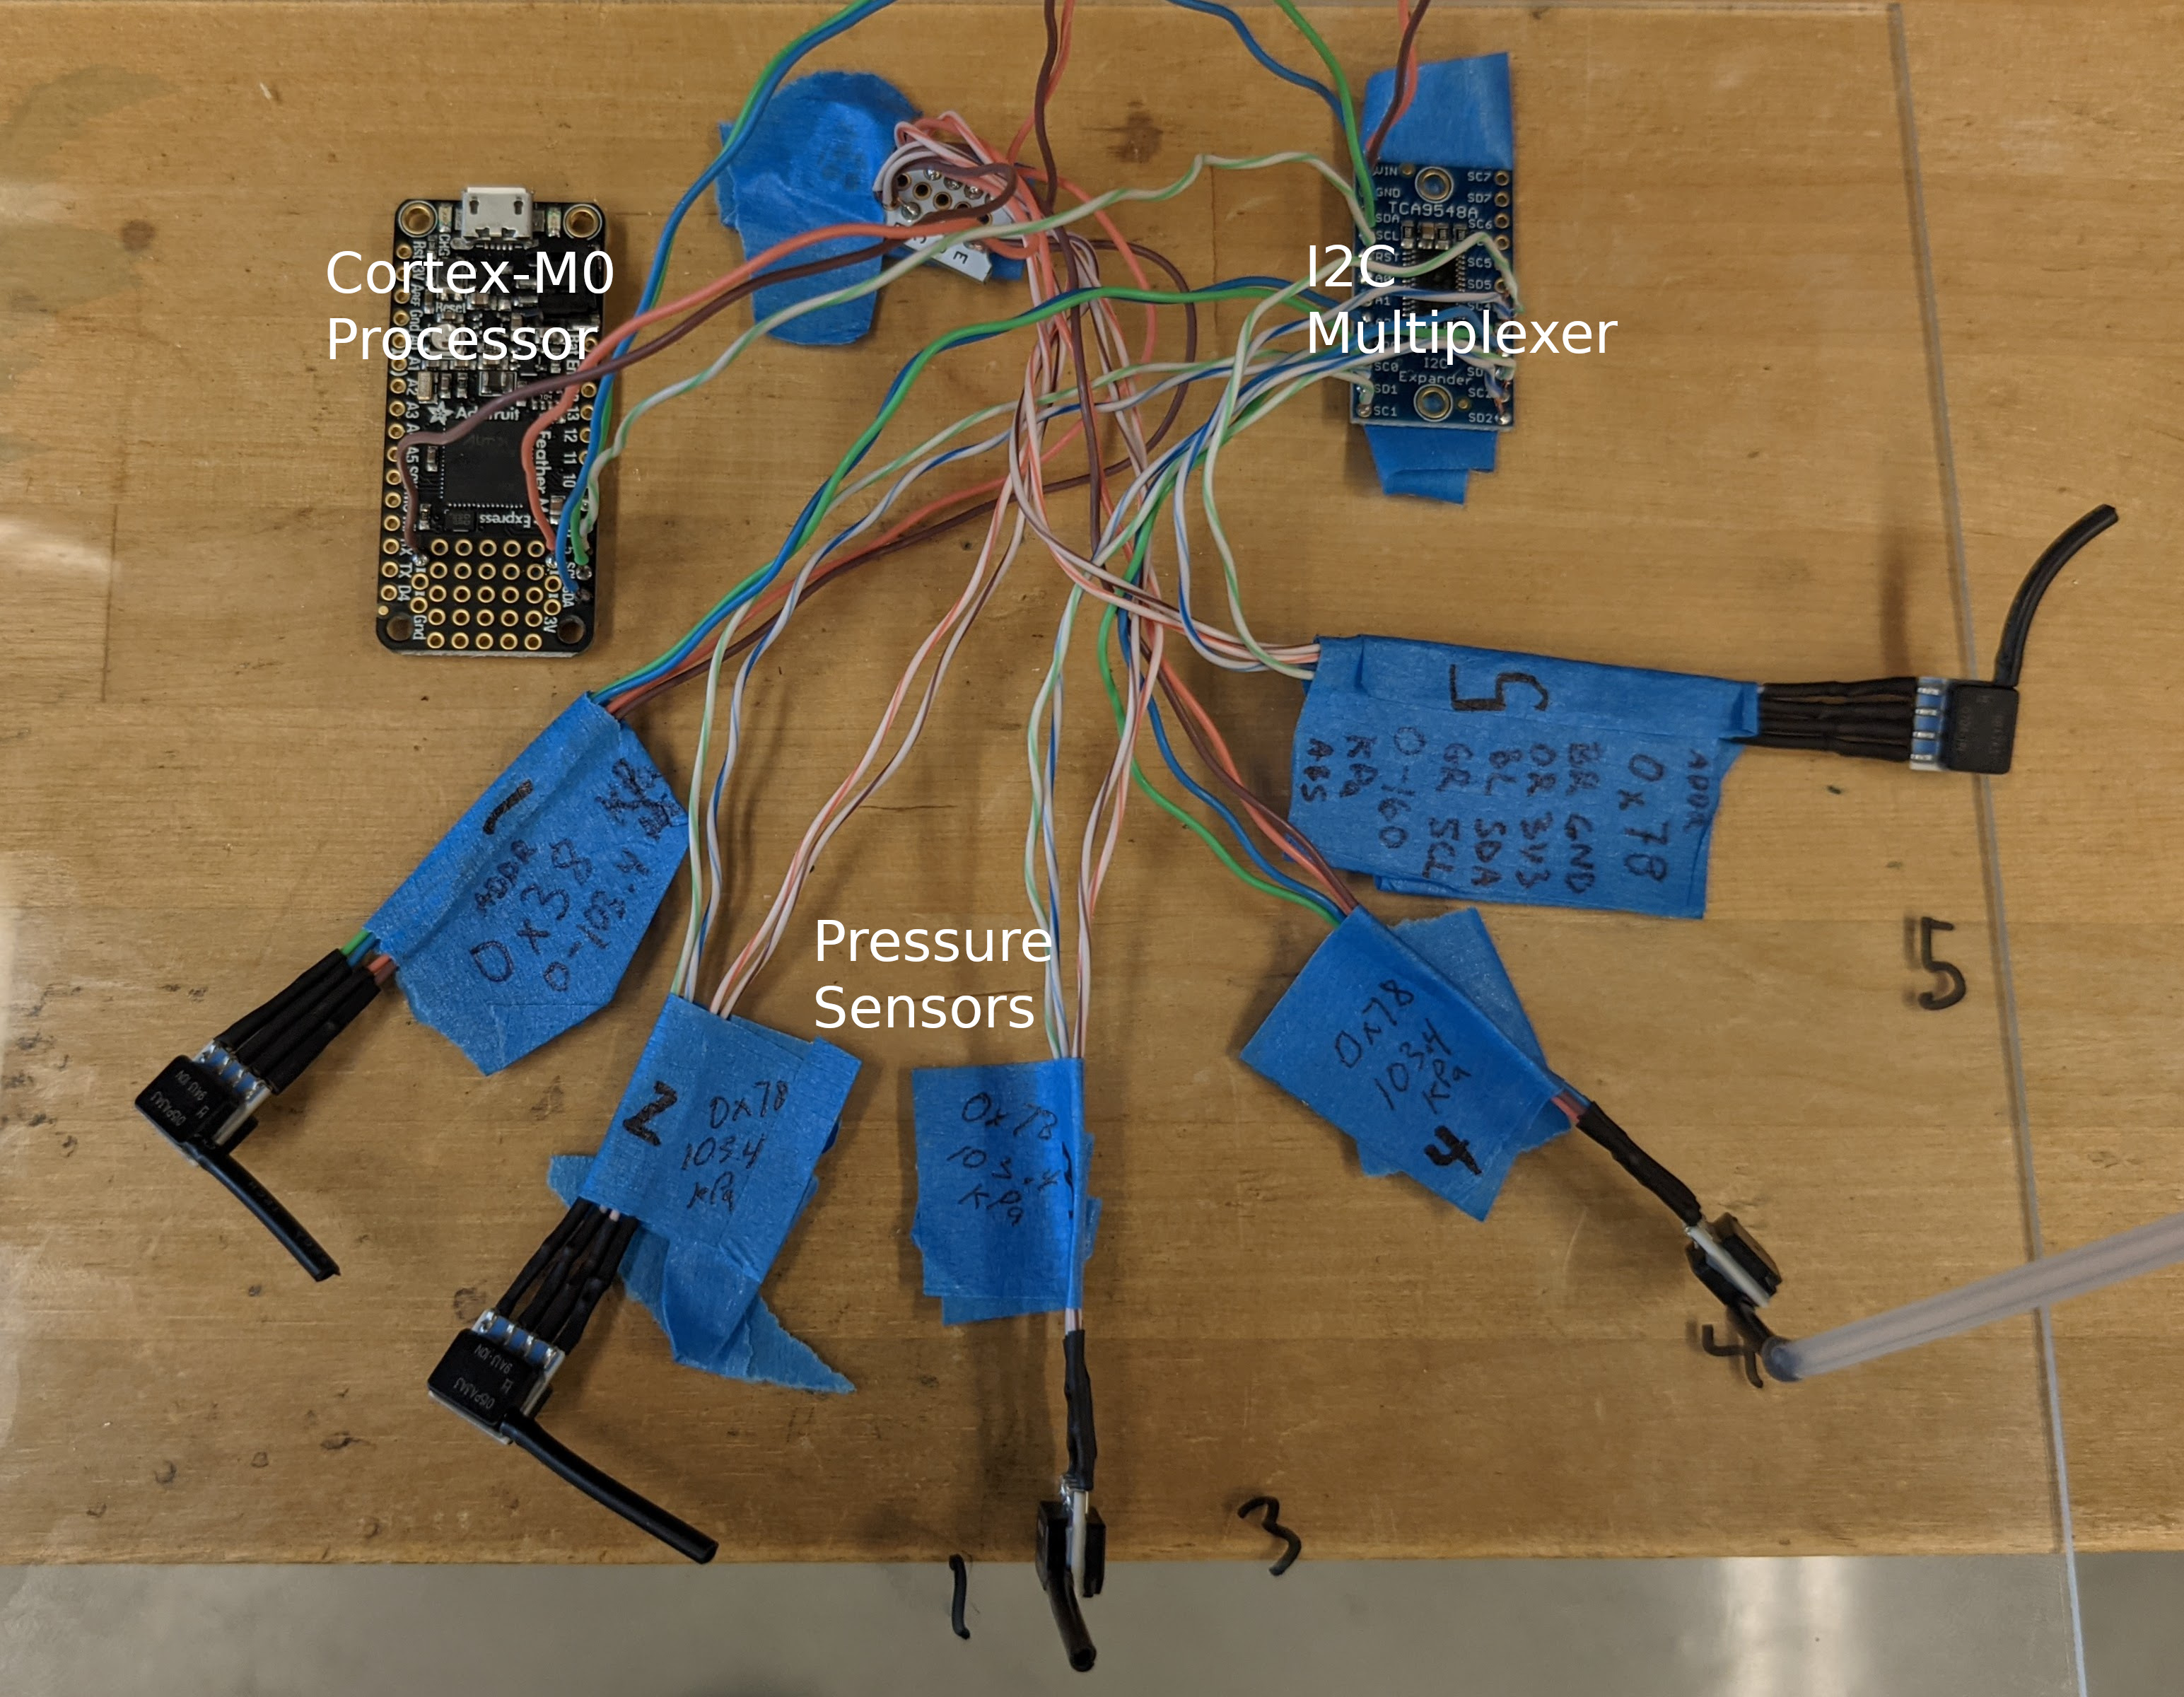
\includegraphics[width=\textwidth]{images/pressure-sensor-testbed-annotated}
	\caption{Testing setup for the pressure sensors.}
	\label{fig:pressure-testbed}
\end{figure}




%\bibliographystyle{plain}
%\bibliography{references}
\end{document}
